\documentclass[a4paper]{report}

\usepackage{listings}
\usepackage{color}
\usepackage[table]{xcolor}
\usepackage{url}
\usepackage[utf8]{inputenc}
\usepackage{newfloat}
\usepackage{todonotes}
% pdfborderstyle to fix the bounding rectangle
\usepackage[pdftex,hidelinks]{hyperref}
% \usepackage[pdftex, pdfborderstyle={/S/U/W 0}]{hyperref}
\usepackage[a4paper,left=4cm,right=4cm,top=3cm,bottom=3cm]{geometry}
\usepackage{emptypage}
\usepackage[page]{appendix}

% For adjusting the spacing between chapters in the TOC
\usepackage{tocloft}
\renewcommand\cftbeforechapskip{3pt}

%\usepackage[hyperref=true,
%			isbn=false,
%			doi=true,
%			url=false,
%			style=alphabetic,
%			urldate=long,
%			urldate=iso8601,
%			natbib=true]{biblatex}
%\addbibresource{thesis.bib}

\usepackage{tikz}
\usetikzlibrary{arrows, decorations.text}
\usetikzlibrary{arrows, decorations.markings}
\usetikzlibrary{shapes,arrows}
% for double arrows a la chef
% adapt line thickness and line width, if needed
\tikzstyle{vecArrow} = [thick, decoration={markings,mark=at position
   1 with {\arrow[semithick]{open triangle 60}}},
   double distance=3pt, shorten >= 5.5pt, 
   preaction = {decorate},
   postaction = {draw,line width=1.4pt, white,shorten >= 4.5pt}]
\tikzstyle{innerWhite} = [semithick, white,line width=1.4pt, shorten >= 4.5pt]

\usepackage{subcaption}
\usepackage{multicol}
\usepackage{xcolor}

\usepackage{pdfpages}

% -------------------------------------------------------------
% Chapter Title
% -------------------------------------------------------------
\usepackage[grey]{quotchap}
\renewcommand*{\chapterheadstartvskip}{\vspace{1cm}}
%  Adding lines below the chapter head
\newcommand*{\ORIGchapterheadendvskip}{}%
\let\ORIGchapterheadendvskip=\chapterheadendvskip
\renewcommand*{\chapterheadendvskip}{%
  {%
    \setlength{\parskip}{0pt}%
    \noindent\rule[.3\baselineskip]{\linewidth}{1pt}\par
  }%
  \ORIGchapterheadendvskip
}

% -------------------------------------------------------------
%  Custom Macros
% -------------------------------------------------------------
\newcommand{\icode}[1]{\mbox{\texttt{{#1}}}}
\newcommand{\fixme}[0]{\textbf{\color{red}FIXME!!}}
% -------------------------------------------------------------
%  Source Code
% -------------------------------------------------------------
\newcommand{\cppfile}[1]{\lstinputlisting[
		basicstyle=\footnotesize,
		breaklines=true,
		language=C++,
		tabsize=2,
		commentstyle=\color{gray},
		keywordstyle=\color{blue},
		stringstyle=\color{red}
	]{#1}}

\lstnewenvironment{cppcode}
    {
		\lstset{
			basicstyle=\footnotesize,
			breakatwhitespace=true,
			breaklines=true,
			language=C++,
			tabsize=4,
			numbers=left,
			numberstyle=\tiny\color{gray},
			commentstyle=\color{gray},
			keywordstyle=\color{blue},
			stringstyle=\color{red},
			xleftmargin=20pt,
			escapeinside={{*@}{@*}}
		}
	}
	{}

\DeclareFloatingEnvironment[fileext=frm,placement={tb},name=Listing]{codefigure}
% \captionsetup[myfloat]{labelfont=bf}

% -------------------------------------------------------------


\title{Correctly Synchronised POSIX-threads Benchmark Applications}
\author{Christos Sakalis}
\date{June 2015}

\begin{document}

\pagenumbering{roman}


\includepdf[pages={1}]{frontpageAndAbstract/frontpageAndAbstract.pdf}
%\null
%\cleardoublepage

\includepdf[pages={2}]{frontpageAndAbstract/frontpageAndAbstract.pdf}

\null
\cleardoublepage
\chapter*{Sammanfattning}
Detta arbete kommer att fokusera på hur prestandan vid körning av program på
en CPU kan ökas. Mer specifikt kommer Store instruktionerna att studeras. Dess
instruktioner osakar ofta stora förseningar i samband med väntan på att data ska
överföras från RAM-minnet till L1 Cachen. Om en out-of-order CPU inte kan hitta
andra instruktioner att jobba med i väntan på datan så kommer dessa cyklar att
bortkastas. För att försöka överkomma denna problematik är en ide att använda
Predictors för att förutspå vilken data som kommer att användas inom en snar framtid
och överföra den till L1 Cachen i förväg. Detta liknar Branch Predictors där CPUn
matas med instruktioner att börjar jobba med baserat på en gissning om branchen
kommer att tas eller inte. Här gissar vi vilka skrivrättigheter som ska överföras till L1 i förväg
istället för vilka instruktioner som kommer efter en Branch. Det är självklart önskvärt
att gissningen är korrekt, men även om den är det så kan vi ha problem, och det är
när ska datan överföras. För sent och vi måste fortfarande vänta eftersom behovet
av skrivrättigheten uppkommer ni den är på plats. För tidigt och skrivrättigheten kan bli avlägsnad från L1
cachen på grund av platsbrist samt att det blir en väntetid för att överföra datan på
nytt när behovet väl uppstår. De senare är också ett slöseri av energi då vi överför
något som kommer att avlägsnas innan användning. Målet med detta masterarbete
är att utröna när data ska överföras för optimal prestanda.
\newpage
\chapter*{Acknowledgment}
I want to thank Alberto Ros from Murcia University and Stefanos Kaxiras from
Uppsala University for presenting the fascinating topic of this thesis to me. Alberto
and Stefanos have given me the required information to carry out this work. They
have also shared their versions of Sniper \ref{subsec:sniper} and Gems \ref{subsec:GEMs}  with me and even
manipulated it with this work in mind. The ideas behind the new policies have been developed in cooperation with Alberto.
\newpage

\pagestyle{plain}

\tableofcontents
\newpage
\listoffigures
 \newpage
\listoftables
\null
\cleardoublepage
\chapter*{Glossery}
\fixme 
\newpage

\pagenumbering{arabic}

\chapter{Introduction}
\label{chap:In}
 \THsec{Motivation}{motivation}
We are always in need of faster and smaller computers that burn less energy. Over
the second half of the twentieth century, the speed of our CPUs (central processing units)
was increased by letting them run at higher and higher frequencies. However, a linear
frequency speed-up causes an exponential increase in energy and heat. In fact, a rule of thumb
is that you are spending as much energy as needed for the computation to cool the
circuit. Since it has become desirable to make smaller and smaller units, it becomes harder and harder
to cool the circuits down. However, software developers still
require more and more of the hardware. When CPUs cannot speed-up
in the same way as before, the CPUs needs to become more effective. That is why
pipelining was introduced into the CPUs. For example, if one instruction takes six seconds to compute, then two instructions will be completed after twelve seconds. If the work were to be divided into three stages where one instruction spends two seconds in each stage, the CPU can then begin working on a new instruction every two seconds. Given this improvement, four instructions are completed in twelve seconds.
Twice the amount of work can be done during a period without increasing the speed
of the CPU and therefore the energy consumption roughly remains the same.
\\ \\
Another opportunity to take advantage of is that computing some instructions, especially
memory instructions (loads and stores) involves long waiting times. If, instead of waiting, other work is computed with the next instructions, one are not affected by the waiting time ultimately. Because the computation of the instructions next in line is started while waiting, this is called out of order execution. It is up to the CPU to decide if the work can be done in another order and still produce the same outcome. 
\\ \\
Like mentioned above computation of memory instructions includes waiting for write permission and that useful tasks can be done while waiting. Still, it is advantageous to decrease the waiting time since there might not always be useful tasks to work on that cover the entire waiting time. This thesis aims to investigate whether we can shorten the waiting time by prefetching the data needed for store instructions in advance. The earlier a data permission is granted, the earlier it is ready to use.
 \THsec{Scope}{scope}
This master thesis introduces and evaluates the three state-of-the-art policies (see \ref{subsec:GPP}) for prefetching permission for the store instruction. There has not been much research focusing on the acceleration of store instructions in particular. The three state-of-the-art policies (OnExecure, OnCommit, and NoPrefetch) are going to be combined in different ways to try to come up with a more optimal policy concerning speed up (number of cycles), number of prefetches, L1 accesses, and power consumption. Furthermore, some of the preparation work concerning editing and understanding traces from benchmark programs are covered as well. 
 \THsec{Related work}{relWork}
The related work for this master thesis is covered in subsection~\ref{subsec:GPP} were the state-of-the-art store prefetch policies are described. 


\THsec{Structure of the report}{structure}

This report consists of eight chapters. 
\paragraph{Chapter \ref{chap:In} - Introduction} This gives a motivation of the work along with its scope. 
\paragraph{Chapter \ref{chap:bg} - Background} This chapter is divided into two parts. The first part covers
the used CPU architecture and related terms to be used throughout the report along with introducing the state-of-the-art policies. The second part covers the methodology employed in this thesis.
\paragraph{Chapter \ref{chap:SettingUpTheTestbed} - Setting Up The Testbed} This chapter can be seen as a continuation of the
second part in chapter \ref{chap:bg}.  Here the modification of existing simulation tools are covered. The trace employed to connect the simulation infrastructure is covered in this chapter.
\paragraph{Chapter \ref{chap:ProposedPrefetchPolicies} - Proposed Store Prefetch Policies} This chapter introduces all store
 prefetch policies that are proposed within the work of this thesis.
\paragraph{Chapter \ref{chap:results} - Results} In this chapter includes graphs comparing the different
 policies with different settings concerning execution times, L1 accesses, useful prefetch, and energy.
\paragraph{Chapter \ref{chap:discussion} - Discussion} Issues with the set up that can have an impact on the results are covered in this chapter.
\paragraph{Chapter \ref{chap:conclusion} - Conclusions} This chapter will offer conclusions about the state-of-the-art and proposed store prefetch policies.
\paragraph{Chapter \ref{chap:fetueredWork} - Future work} This chapter presents ideas on future work that can be
built upon the work of this thesis.


\chapter{Background}
\label{chap:bg}
This chapter is divided into two sections. The first one, \ref{sec:ThB} Theoretical Background,
describes a simple CPU architecture which focuses on the parts used
for executing memory instruction, i.e., stores. It is followed by an introduction of
the three state-of-the-art prefetching strategies. Section \ref{sec:siminf}  goes through the
workflow of this thesis and introduce the tools that are used, modified or created, as
well as how they are combined.
\THsec{Theoretical Background}{ThB}

\THsub{A theoretical Architecture}{TA}
\begin{figure}[h]
\centering
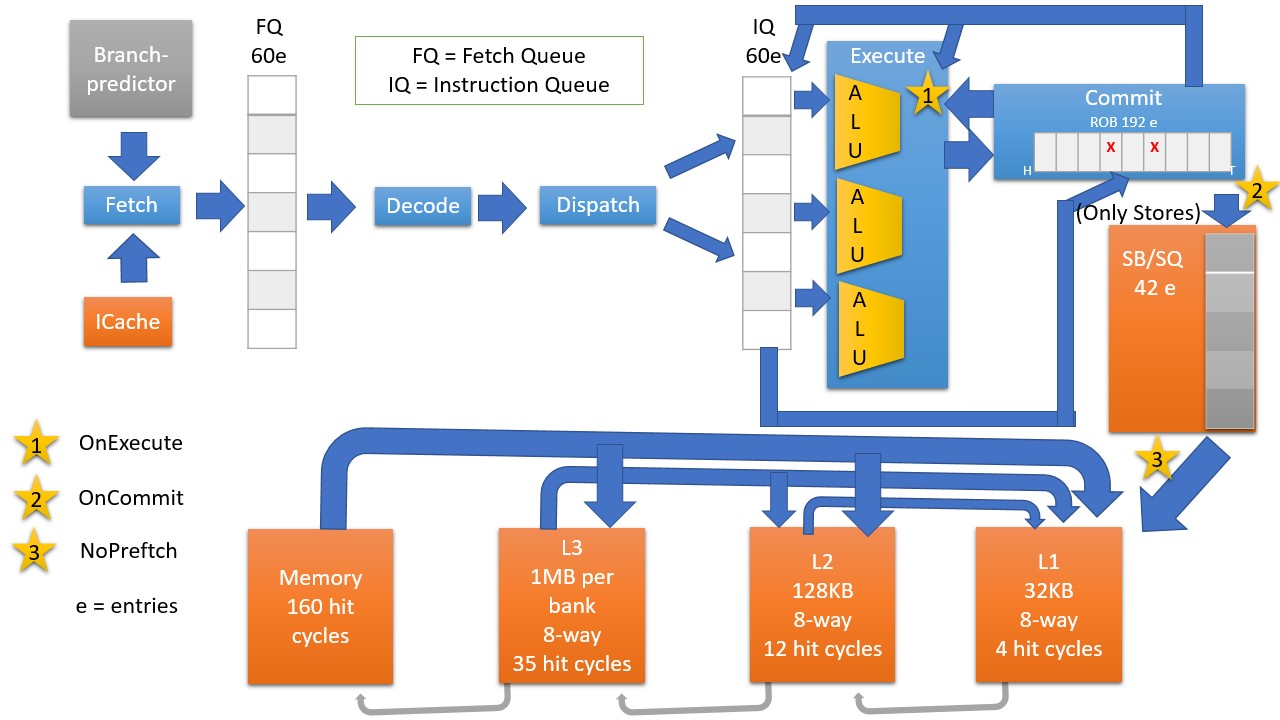
\includegraphics[width=12cm]{figure/thoeratical-arc.jpg}
\caption{Our architecture}
\label{img:arc}
\end{figure}
The image \ref{img:arc} shows architecture in use. This image symbolizes almost all
the features and parts of the CPU that are going to be discussed and analyzed from different
perspectives. If there is a picture that you should keep in mind when reading this
report, then this would be it. The stars symbolize where a prefetch is issued for the
three state-of-the-art store prefetch policies evaluated in this thesis (section \ref{subsec:GPP}). The structure is the one used for the
simulated CPU (see section \ref{sec:arc}). In modern CPU’s there is often more than one
core which all have a processor pipeline with several stages. The pipeline is split into
stages to increase the throughput of executed instructions. One can compare it with
a car factory where the cars travel on a conveyor belt through different stations and
at each station, something is installed within the car, i.e., seats, wheels or the engine.
\\ \\
The simulated CPU has a seven stage pipeline (for simplicity Decode and Allocation is here combined). Some key parts of the CPU are introduced while covering these stages. One thing to mention before moving
on is that the CPU executes instructions out of order but with the promise that the effect
is always like as if the instruction executed in order.
 \\ \\

\THstage{Fetch}
A new instruction (see \ref{sec:trace}) is added to the processor. In the most comen case the
next instruction is brought in from the \THnewWord{I-cache} (Instruction cache). I-cache is
an L1 cache \THnewWord{cache} that holds the instructions to be executed shortly.
The CPU has a \THnewWord{PC} (program counter) which keeps track of the address of the current
instruction fetched. When fetching the next instruction, the PC
increments by the length of the current instruction. caches will covered in \ref{subsubsec:memcache}.
Different loops are used in programming, and a loop tells us if we should go
back to the beginning of the body of the loop or if the loop should terminate
and the lines below it should execute. A CPU cannot, for example, execute C code,
it needs to compile first. A compilation is a translation from code to instructions
within the instructions set that are supported by the CPU in question. A loop is compiled to a branch instruction which has a target instruction address
and the condition to be satisfied if the branch is taken (take one more lap in the
loop). The problem is that we want to continue to bring in new instructions before
the condition is computed, but which instructions are next? Here
the \THnewWord{Branch predictor} come to use since it predicts the outcome of a branch and makes the CPU
able to load instructions based on that prediction. If a branch is taken the PC is set
to the branch target address. If a prediction turns out to be wrong, the CPU has to remove
the work and all the side effects produced by the wrongly executed instructions.
Fetched instructions are placed in the fetch queue (our has 60 entries).
\THstage{Decode (and Allocation)}
The instruction (from the instruction queue) will here be interpreted. In the Allocation, phase recurses like entries in the Issue queue (IQ), Reorder buffer (ROB), and Store buffer (SB) are received~\cite{CPUbook}. The two later buffers are introduced later on.
\THstage{Dispatch}
In this stage, we take care of dependencies. If we want to add two numbers and
then multiply the result with a third number, then the addition has to be finished
before the multiplication can be executed. Thus the multiplication has a dependency
on the addition. If we also have to store the result of the multiplication, then the
multiplication needs to be computed before we can store the result of it. This gives a
dependency between the store and the multiplication. When the dependencies have
been worked out, the instructions will be put in the \THnewWord{Instruction queue} (IQ) (which
has 60 entries as well).

\THstage{Execute}

Here is the arithmetic computation performed. It takes place in on of the arithmetic logic units (ALUs), for the store instructions this means calculating the memory address. The instructions may be executed out-of-order. 

\THstage{Commit}
Commit is the last step of the pipeline, and it shares the ROB (ReOrdering Buffer),
with 192 entries, with some of the previous stages. This buffer puts the out-of-order executed instructions back into
order. Given the size of the ROB, it is possible to execute 191 instructions ahead
while waiting for an instruction to finish. When all instructions in a sequence are
done, they can leave the pipeline. The {\color{red}x} in figure \ref{img:arc} illustrates a squashed instruction.
If a branch prediction turns out to be wrong, then we need to squash all the instructions
that should never have been executed but have been based on that incorrect prediction.

When the addition, with the sum of two number multiplied by a third number, is done and the result is added to the ROB, the multiplication
instruction in the \THnewWord{IQ} (Instruction Queue) gets informed that its dependent instruction
is done (the arrow from ROB to IQ in figure \ref{img:arc}). Finally the arrow from ROB to
ALU provides the result from the addition to the multiplication.
\THstage{SB}
Every instruction takes the path that has been described until now, now
we continue to describe the way that only store instructions take. When a store instruction
leaves the ROB, it goes to the \THnewWord{store buffer} (which can also be called store queue).
The store instruction is now represented by the memory address to be fetched
and the data to be stored. The buffer is FIFO-ordered (first in first out), this means that the first
store in the buffer waits for its data to be ready in the L1 cache (see \ref{subsec:TA}) and blocks all operations behind it in the buffer. The store buffer
interacts only with the L1 cache.

\THsubsub{Memory and caches}{memcache}
The memory structure (in the center of figure \ref{img:arc}) is, of course, an essential part when talking
about store instructions. We begin with the main memory that has a storage capacity
of some gigabytes, a latency of 160 cycles if a hit, and is located on the motherboard. Then
we have the caches, which are placed on the CPU chip. A cache is a quick and small
memory unit in which the data that are likely to be used soon is placed.
In this case, we have three caches which are named L1 (32kiB 8-way 4 hit cycles), L2 (128kiB
8-way 12 hit cycles) and L3 (1MB per bank 8-way 35 hit cycles). L stands for
level, and the higher the digit, the bigger the cache is and the further away from the
core it is located. A bigger cache means that it takes a longer time to find specific data
in it. The time is measured in \THnewWord{cycles}, and in every cycle, something can occur in the CPU, i.e., an instruction can be placed in FQ and/or another one can be placed in the ROB.
If our CPU runs in a frequency of 2.2 GHz, there are:

$$ 2.2 \times 1000^3 = 2.2 \times 10^9 cycle / second$$

Given that one cycles takes:

$$ \frac{1}{2.2 \times 10^9 } = 2.2 \times 10^{-9}s = 2.2ns$$

This gives us that it takes $4 \times 2.2 = 8.8ns$ to retrieve data from the L1 cache. A
cache keeps copies of needed data, and the data are saved in different regions in
within the cache depending on the address of the data. The number of ways a cache has
is the same as the number of data shanks in every address range that can be kept simultaneously
within the cache. The higher number of ways means that it takes a longer time to determine
if a specific data is present in the cache. The smaller number of ways the higher risk of conflict misses, that is when the cache runs out of places for data from a specific
address range. Our coaches are all 8-ways which means that a piece of data can be
in one of eight places (if it is in the cache) and that a cache can hold no more than
eight data chunks from a given address range. The Icache is like another L1 cache
that only holds instructions while the L2 and L3 cache hold both data and instructions.
When data loads into the L1 cache from the main memory, it often loads
to all the other caches at the same time.


\THsub{State-of-the-art prefetch policies}{GPP}
The question for this master thesis is when to prefetch permission into the L1 cache to
minimize the time a store instruction has to wait in the first place of the store buffer. 
Three approaches were already implemented in the Gems simulator \ref{subsec:GEMs} at the beginning of this thesis and are covered in the literature,  these will
be described, and their pros and cons while be mentioned below, based on the architecture
introduced in section \ref{subsec:TA}. These three policies are also referenced to as "the basic three policies." The "stars" mentioned in the paragraph headings
are the once in figure \ref{img:arc}
\THpar{OnExecute (star 1)}{ONEX} OnExecute \cite{ONEX} is the earliest and most speculative store prefetch policy, where the
operation to bring memory into the L1 cache is issued within the execute stage. It
ensures that the data arrives in L1 before it is needed, i.e., its instruction in at the head of the store buffer. The downside is that several events which impact on the data to be prefetched can
occur. First, if the store instruction is affected by a branch, that branch can
be mispredicted which means that we waste energy and space in the small L1 cache
by bringing in unneeded data. Bringing in data to a cache can cause eviction of
other data. When a store instruction takes first place in the buffer and finds that
its data have been evicted from the L1 cache it has to wait for the data to be brought
to the L1 again. It might take less time since the data can be left in the L2 cache and be brought from it instead of the main memory.
\\ \\
Given that the prediction
is right we might still be in trouble since when we issue the prefetch, the instruction
has to finish the pipeline and passes through the queue in the buffer. This process might
take a long time. During this time the data can have arrived in the L1 cache and been
evicted due to lack of space. This lack of space is due to more data have been prefetched from the point in
time it arrives in L1 until the instruction is at the head of the store buffer. Prefetching to early
can also become a vulnerability since malicious software can cause a prefetch of illegal data
before the core figures out that it is illegal, and when it does the data have already
been exposed. To conclude: one can say that this alternative is the best if nothing
goes wrong, but many things can go wrong. 

\THpar{OnCommit (star 2)}{ONCO} In this case, the prefetch is issued in the commit stage (when passing
the store to the store buffer). Unneeded data will not be
prefetched. There is still a possibility that the data will be brought in to the L1 cache and evicted
due to lack of space, as described in the previous paragraph. Prefetching
data on commit might still mean that the instruction may be waiting in the head
of the store buffer. This waiting can, in the worst case, fill up the entire buffer which can stall the
processor, i.e., block it from executing any other instruction. Intel 64 and IA-32 Architecture \cite{ONCO} uses OnCommit. They do not use the name OnCommit, but they
quickly describe a load prefetch with the following sentence: ”Reading for ownership
and storing the data happens after instruction retirement and follows the order of
store instruction retirement.”. ”Reading for ownership” is the same as prefetch with
write permissions and ”instruction retirement” is another name for ”instruction commit.” 
To conclude, OnCommit is the one in the middle between the two extremes,
OnExecute (star 1) and NoPrefetch (star 3).

\THpar{NoPrefetch (star 3)}{NOPF} Here we have no prefetch, the data will be brought into the
L1 cache when the instruction is in the head of the store buffer. All data brought will be
needed and not evicted before use. This waste no energy in brought unneeded data. The downside of this is that every
instruction will be blocking the buffer for a long time waiting on its data to become
available in the L1 cache. The risk for filling up the buffer and stall the processor
(see \ref{subsubsec:memcache}) is therefore high.
\\ \\
To conclude: this is the most energy efficient, but also the most time-consuming trade-off. Upon analyzing the source code of Gem5 \cite{gem5} it was discovered
that NoPreftch was the default implemented policy. During the work of this thesis, new prefetch policies were implemented as well.

\THsec{Simulation infrastructure}{siminf}
Below the tools that have been used for this thesis are
covered. The tools that have been modified or created within the work of this master thesis
are to be found in chapter \ref{chap:SettingUpTheTestbed}.
\THsub{Benchmarks}{benchmarks}
To examine how a CPU behaves and how a certain store prefetch policy will work
one has to run, or in this case, simulating the run of a program. These types of programs are often called
benchmarks. For this work, the SPEC CPU \textcopyright 2016 industry-standardized benchmark
suite \cite{specCpu} was used. It is designed to stress both the CPU and the memory subsystem, and it consists of 55 different benchmark programs that have been used to evaluate
different prefetch policies.
\\ \\
One million instructions from every benchmark are going to be simulated. A warmup of 10\% is used, i.e., the measurements will start after the execution of the first one hundred thousand instruction. A warmup is caused in the begging of an execution since there will always be a miss in the caches and we do not want that phase to affect the result.
\THsub{Sniper}{sniper}
Sniper is a parallel, high-speed and accurate x86 simulator with support for multicore
according to their website \cite{sniper}. Sniper takes two things as input, a bunch of configurations
that describes the architecture to simulate, and a command line with the call to
the application which we want to simulate, for example, one of the programs in 2.2.1.
Sniper can then produce graphs and other documents that describe and measure the
simulation of the chosen program on the chosen CPU configuration. Two examples of
plots that can be generated are CPI stacks \cite{cpi} and energy stack  (bar diagrams
with one bar per thread in the program). These bars are divided into different regions
based on the percentages of time or energy spent in that region. The region can be:
Ifetch, mem-l1, mem-l2 or branch.
\THsub{GEMS}{GEMs}
The Wisconsin Multifacet Project at the University of Wisconsin has released a General
Execution-driven Multiprocessor Simulator (GEMS). The simulator is written in
C/C++ and it is an open-source software. The version used in this work was provided
by my supervisor (Alberto Ros) who had implemented the three basic prefetch
policies (NoPrefetch, OnCommit, and OnExecute) along with one that he has come
up with but not yet published (OnNonBSpeculative). He has also created support for the changes
to the traces in Sniper that was done during this thesis (see \ref{subsec:sniper}). Support for the
policies to be proposed in this work was implemented based on the received source
code.
GEMS was modified to take a path to a folder containing traces (like in \ref{sec:trace}), an array of configuration
settings (see \ref{sec:conf} and \ref{sec:ThB}) and a path for writing the output stats-file. A
stats-file consists of around 2000 lines and is divided into two parts: A configuration part where you find the information given to GEMS in the configuration array and
a Stats part with many measurements like the number of cycles and the number of
accesses to the caches.

\input{applications.tex}

\chapter{Results}
\label{chap:results}

This chapter shows the results of the different filters and store prefetch policies concerning; execution times, number of L1 accesses, number of store prefetches and
energy consumption, which are referred to as metrics. This chapter is divided in four
sections, one for each set of techniques (introduced in chapter \ref{chap:ProposedPrefetchPolicies}) and the State-of-the-art ones (see \ref{subsec:GPP}). In each of these sections, there is one subsection for each
metric. Every subsection presents the average values for each compared policy combination in a table. This table follows by a graph with the values of all benchmark
for all compared policy combination. The values are given in percentages normalized
to OnCommit. Finally the five benchmarks that benefit the most and the least from
a certain policy combination compared with OnCommit are presented.
\THsec{State-of-the-art policies}{base}

First, the state-of-the-are store prefetch policies will be analyzed:
\begin{itemize}
    \item NoPrefetch
    \item OnExecute
    \item OnCommit
\end{itemize}
\resExtime
\avgTable{extime}{run1-0-avg}{execution time}{}
This table shows the impact of the prefetched policies on average runtimes. When
using any type of prefetch policy it will roughly cut the runtime with a third (for
OnCommit and OnExecute). These results tell us that bringing data into the L1
cache for store instructions is a bottleneck. Still, it is not just to prefetch data for
all store that may be executed. If comparing OnExecute and OnCommit, one can
see that OnExecute is 2.35 \% units slower. Since OnExecute issues there prefetches earlier they will, therefore, prefetch more data that later will turn out to not be used. Unnecessary prefetch slows down the execution, and should be minimized.
\fullTable{extime}{run1-0-full}{Execution time}
\toplist{extime}{run1-0}{execution time}{OnExexcute}
The table above presents the number of percent units in terms of the number of
cycles for a particular benchmark when comparing OnExecute and OnCommit. Gcc
3 and Gobmk 4 gain over 20 \% in reduced number of cycles while running OnCommit
(being less aggressive with the prefetch). On the other hand, OnCommit is increasing the number of cycles for Omnetpp and CactusADM with a 20 \% units. The ones that
goes well with OnExecute are the ones that do not have so much need of prefetching,
makes the best results for NoPrefetch. The ones that are very sensitive to prefetch
go well with OnExecute.
\resAcc

\avgTable{L1}{run1-1-avg}{number of L1 accesses}{}
This is an interesting table which shows the amount of unnecessary work caused
by prefetching. NoPrefetch does, as the name suggests, no prefetches which mean that
all L1 accesses are caused by store instructions that write to the cache. Everything
above 84.82\% is unnecessary work and will waste energy. OnExecute does as expected
more accesses than OnCommit since it prefetches earlier and is more speculative.

\fullTable{L1}{run1-1-full}{Number of L1 accesses}
\toplist{L1_1}{run1-1}{number of L1 accesses}{OnExexcute}
The table shows that OnCommit decreases the L1 accesses for all but two of
the benchmarks and the difference can be over 90\% units (Bzip2 1 and Bzip2 2).
This behavior shows once again that an early prefetch triggers unneeded accesses to
 the L1 cache. It is interesting that Soplex 1 has more accesses for OnCommit than
OnExecute and this might be something to investigate further.
\resSp
\avgTable{sp}{run1-2-avg}{number of store prefetches}{}
The number of store prefetches confirms the behaviors and conclusions drawn from the tables over execution times and L1 accesses. NoPrefetch does not store prefetches
while OnExeute does it the most. 299.72\% units more than OnCommit. This is also
what to expect since OnExecute is more speculative then OnCommit. Another thing
to notice here is that sometimes after commit, the store instruction is already at the
head of the Store Buffer, and therefore it issues the write instead of the prefetch. The
effect is equivalent with NoPrefetch.
\fullTable{sp}{run1-2-full}{Number of store prefetches}
\toplist{sp1}{run1-2}{number of store prefetches}{OnExexcute}
OnExecute issues more store prefetches then OnCommit for all the benchmarks
except Bwaves which has the same number of prefetches for OnCommit and OnExecute.
\resEnergy
\avgTable{energy}{run1-3-avg}{energy consumption}{}
This table shows the energy consumption of each prefetch technique. First of all,
NoPrefetch consumes the smallest amount of energy while OnExecute consumes the
most. This consumption comes from unnecessary prefetches. It is also worth noting
that if using OnExecute instead of OnCommit the number of cycles decreases by 2.35\%
units, but the energy consumption increases with 33.13\% units. Using OnCommit
instead of NoPrefetch burns 9.05\% units more energy but that gives a speedup of
46.5\% units. A prefetch policy can pay off in decreased energy consumption, but if getting too far in prefetching the loss concerning increased energy consumption can be huge.
\fullTable{energy}{run1-3-full}{Energy consumption}
\toplist{energy}{run1-3}{energy consumption}{OnExexcute}
Using OnCommit rather then OnExexute saves much energy for many benchmarks. Finding Bizp2 in the lead when it comes saving energy is no surprise since it is in the lead when it comes to decreasing prefetches and L1 accesses. This correlation will also explain why Milc increase a bit in energy consumption while using OnCommit instead of OnExecute. Longer execution time will also increase the energy consumption.



\THsec{Techniques to reduce speculation effect}{reduce}
Second, all prefetch policies from state of the art and the following three new ones
will be analyzed:
\begin{itemize}
    \item OnNonBSpec (OnNonBSpeculative)
    \item OnExecute with Re-Execute
    \item OnNonBSpec with Re-Execute
\end{itemize}
\resExtime
\avgTable{extime2}{run2-0-avg}{execution time}{}
OnNonBSpec seems to be the fastest one, 3.34\% units faster then OnCommit.
It makes a difference not to prefetch stores that are affected by a branch. The Re-Execute filter affects OnExecute with 1.22\% units but OnNonBSpec with only 0.08\%
units.
\fullTable{extime2}{run2-0-full}{Execution time}
\toplist{extime2}{run2-0}{execution time}{OnNonBSpec with Re-Execute}
Most of the benchmarks benefit from using OnNonBSpec with Re-Execute, in the
lead, CactusADM (with 14.97\% units) and Omnetpp (with 11.05\% units). The ones
that loses by using OnNonBSpec with Re-Execute does so by under two percent.
\resAcc
\avgTable{L12}{run2-1-avg}{number of L1 accesses}{}
 OnNonBSpec does 4.04\% units less L1 accesses then OnExectue. Re-Execute decreases the L1 accesses with 3.60\% units used on OnExecute and 0.95\% units used on
 OnNonBSpec. The difference can be explained by OnNonBSpec removing some of the
prefetches that ReExecute also will remove. The total numbers tell us that OnNonBSpec with Re-Execute has the lowest number of L1 accesses apart from OnCommit
 with 100.00\% against 118.26\% (OnExectue with Re-Execute). 
\fullTable{L12}{run2-1-full}{Number of L1 accesses}
\toplist{L12}{run2-1}{number of L1 accesses }{OnNonBSpec with Re-Execute}
In this table OnBSpec has more L1 accesses for all benchmarks except Spolex.
Bzip2 1 and Bzip2 2 have over ninety percent more accesses and are the two benchmarks that have the highest increase.
\resSp
\avgTable{sp2}{run2-2-avg}{number of store prefetches}{}
OnNonBSpec decreases the number of store prefetches by 57.60\% units compared
with OnExecute. Re-Execute is also decreasing the number of prefetches with 15.64\%
units used on OnExecute and 7.68\% units used on OnNonBSpec. The difference can
be explained by OnNonBSpec removing some of the prefetches that Re-Execute also
will remove. The total numbers tell us that OnNonBSpec with Re-Execute has the
lowest number of L1 accesses apart from OnCommit (and NoPrefetch) with 336.54\%
against 384.08\% (OnExectue with Re-Execute).
\fullTable{sp2}{run2-2-full}{Number of store prefetches}
\toplist{sp2}{run2-2}{number of store prefetches}{OnNonBSpec with Re-Execute}
OnNonBSpec with Re-Execute does more prefetches then OnCommit for all benchmarks except Bwaves, which stays the same. In first place is bzip2 1 which increases the prefetch by 4687 percent units.
\resEnergy 
\avgTable{energy2}{run2-3-avg}{Energy consumption}{}
What to notice here is that OnNonBSpec burns 22.89\% units less energy then
OnExecute. Re-Execute decrease the energy consumption with 3.24\% units used on
OnExecute and 0.82\% units used on OnNonBSpec. OnNonSPec with ReExecute gets
109.42\% units, which is 9.42\% units more than OnCommit.
\fullTable{energy2}{run2-3-full}{Energy consumption}
\toplist{energy2}{run2-3}{energy consumption}{OnNonBSpec with ReExecute}
OnNonBSpec with Re-Execute can decrease the energy consumption for some
benchmarks with only a few percent units, and the best is Gcc 2 with 4.37 \% units
less energy consumption. However, for some other benchmarks like Bzip2 1 and
Bzip2 2, the consumption is increased, in this case by around 90 \% units. To see
these two benchmarks consume the most energy is not a surprise since they are high
on L1 accesses and store prefetch.

\subsection{Conclusion}
OnNonBSpec with Re-Execute is the fastest store prefetch policy with a speed-up of 3.42 \% units compared to OnCommit, but it burns 9.42 \% units more energy. The
question to ask is if an energy increase with 2.75 \% units is worth a speed-up of 1 \%
units. It is likely to believe that the answer will differ with the type of machine and
application. OnNonBSpec with Re-Execute will be kept together with the three stateof-the-art policies as the reference for the future once. The new filters and policies to
be tested will all be put on top of it. All the polices (except NoPrefech) still consumes
more energy then OnCommit, the techniques introduced next will aim to reduce this
consumption.
\THsec{Techniques to filter unnecessary prefetches}{filter}
In this section sameCachLine and PCbasedPredictor (PCbased) are introduced. The  digit after PCbased denotes the buffer size, the number of entries is two to the power
of the digit. Tests have been conducted with PCBased2, 4, 6, 8, 10 and 16 but as it
turns out 2 behaves in the same way as 4, and 8 the same as 6, and so on in all four
metrics (execution time, L1 accesses, number of prefetch and energy consumption).
Therefore, to reduce the number of configurations in the tables of this section, only
buffer sizes 2 and 8 are used. The new configurations, based upon OnNonBSPec with
Re-Execute, are:
\begin{itemize}
    \item OnNonBSpec with sameCacheLine
    \item PCbasedPredictor 4
    \item PCbasedPredictor 4 with sameCacheLine
    \item PCbasedPredictor 8
    \item PCbasedPredictor 8 with sameCacheLine
\end{itemize}
\resExtime
\avgTable{extime3}{run3-0-avg}{execution time}{* with sameCacheLine}
 SameCacheLine has a little slowdown on OnNonBSpec (the best from 5.2) with
0,06\% units and 0.08\% units, on PCbasedPredictor (2 and 8). One hypothesis for this
is that loading the same permissions twice in a short manner of time will not be an
issue since the memory-subsystem will quickly realize that the requested permission
is already in the L1 cache. Therefore blocking the second prefetch of a cache line a
bit earlier will not have a big impact, at least on the execution time.
\\ \\ 
PCbased 4 and 8 have the same numbers 96.96\% without sameCacheLine and 96.88\% with. These results can be compared to OnNonBSpec with its 96.64\%, with sameCacheLine. Iterate over a buffer as in PCBasedtakes time, so the advantage of doing
that has to pay more at runtime. Otherwise, it will end up with a slowdown as here.

\fullTable{extime3}{run3-0-full}{Execution time}
\toplist{extime3}{run3-0}{execution times}{OnNonBSpec with SameChacheLine}
Here OnCommit is compared with OnNonBSpec with Re-Execute and SameCacheLine, since its the best one concerning execution time among the new one for
this section. Some benchmarks seem to benefit from OnNonBSpec with Re-Execute and SameCacheLine while others do not. The absolute value of the one benefiting
the most from OnNonBSpec with Re-Execute and SameCacheLine is higher than the
one losing the most ($| − 16.10| > |6.58|$).
\resAcc
\avgTable{L13}{run3-1-avg}{number of L1 accesses}{* with sameCacheLine}
PCbasedPredictor 4 and 8 have the same number of L1 accesses (105.76\%). SameCacheLine improves both on OnNonBSpec with 1.15\% units and on PCbasedPredictor (4 and 8) with 0.73\% units. PCbasedPredictor (4 and 8) with SameCacheLine
becomes the closest one to OnCommit with it is 105.03\%.
\fullTable{L13}{run3-1-full}{Number of L1 accesses}
\toplist{L13}{run3-1}{Reduce speculation the benchmarks which number of L1 accesses are affected the most (in number of percent)}{OnNonBSpec with SameCaceLine}
This table shows us that OnNonBSpec with Re-Execute and SameCacheLine decreases the L1 accesses for only two benchmarks, Milc (-3.52\% units) and Gcc 2 (0.17\% units). Hmmer is the benchmark that has the greatest decrease of L1 accesses
26.20\% units.
\resSp
\avgTable{sp3}{run3-2-avg}{number of store prefetches}{* with SameCacheLine}
The store prefetches shows roughly the same thing as L1 accesses (see table 5.19).
PCNessary (4 and 8) gives the same percentage without SameChaheLine, 155.16\%,
and with, 151.95\%, a difference of 3.21\% units. SameCacheLine also improves OnNonBespec with 6.02\% units. PCNessary (4 and 8) with SameCacheLine is once again
closest to OnCommit with it is 151.95\%.
\fullTable{sp3}{run3-2-full}{Number of store prefetches}
\toplist{sp3}{run3-2}{number of store prefetches}{OnNonBSpec with SameChacheLine}
All benchmarks do more store prefetches then OnCommit when using OnNonBSpec with Re-Execute and SameCacheLine, except for Bwaves which stays the same.
The two benchmarks that increased their store prefetches the most are Libquantum
(247.48 percent units) and Bzip2 5 (240.84 percent units).
\resEnergy
\avgTable{energy3}{run3-3-avg}{energy consumption}{* with sameCacheLine}
There is no surprise that the energy corporation looks the same as L1 access and
store prefetches. PCNessary (4 and 8) has the same percentages, without, 103.91\%,
and with SameCacheLine and it is decreased with 0.66\% units to 103.25\%. OnNonBSpec drops with 0.78\% units to 108.64\% with SamecacheLine. However, it is not
enough to beat PCBasedwith SameCacheLine.
\fullTable{energy3}{run3-3-full}{Energy consumption}
\toplist{energy3}{run3-3}{energy consumption}{OnNonBSpec with SameCacheLine}
 Four of our benchmarks saves energy by using OnNonBSpec with Re-Execute and
SameCacheLine. The one saving the most is Milc with its 4.47\% units. Hmmer does 
must store prefetches and consumes the must energy, 22.87\% units more than for
OnCommit.
\subsection{Conclusion}
SameCacheLine does not get affect at all on the execution time, but it saves energy
by removing L1 accesses and prefetches. Therefore SameCachLine should be added
to the currently best policies. PCbasedPredictor gives the same runtime and burns
the same amount of energy for both sizes 4 and 8. It is cheaper and more efficient
to have a buffer with $2^4=16$ entries then $2^8=256$ entries and therefore PCBased4
does and OnNonBSpec, both with SameCacheLine will be compared.

    \begin{table}[H]
\centering

\begin{tabular}{ |l|l|l| }
\cline{2-3}
\multicolumn{1}{ c| }{} 
& Execution time & Energy  \\  \hline
PCBased 4& 96.88 & 103.25  \\  \hline
OnNonBSPec & 96.64 & 108.64  \\  \hline
Difference & 0.24 & 5.39  \\  \hline
\end{tabular}
\caption{Comparation between PCBased 4 and OnNonBSpec, both with SamecacheLine. }
\label{quickcompPC4vsONBS}
\end{table}
In the table above \ref{quickcompPC4vsONBS} shows that OnNonBSpec is fastest but PCNessary 4 burns
less energy. So the choice is based on what the biggest concern might be in a given setting, time or energy. PCbasedPredictor 4 is a bit slower, 0.24\% units, but the energy
savings is much higher (5.29\% units) therefore should PCNessary 4 with SameCacheLine be considered the best policy of this section and be together with the basic three
the ones to be taken to the next section.
\THsec{Techniques for timelLiness}{timelines}
In this last section the following policies are added, which all build upon PCbasedPredictor 4 with Re-Execute and SameCacheLine:
\begin{itemize}
    \item PCbasedPredictorTimeliness2 4 (PCbasedTL2 4)
    \item PCbasedPredictorTimeliness2 8 (PCbasedTL2 8)
    \item PCbasedPredictorTimeliness3 4 (PCbasedTL3 4)
    \item PCbasedPredictorTimeliness3 8 (PCbasedTL3 8)
\end{itemize}
\resExtime

\avgTable{extime4}{run4-0-avg}{execution time}{* with reExecute and SameCacheLine}
PCNessaryTimeliness3 has longer run times, 97.89\% for size 4 and 97.51\% for size 8,
iterate over a bigger buffer takes more time for PCNessaryTimeliness3.
\fullTable{extime4}{run4-0-full}{Execution time}
\toplist{extime4}{run4-0}{execution time}{PCbasedPredictor~4*}
PCbasedPredictor 4 speeds up at least five benchmarks with Mlic in the top (7,84\%
units). On the other hand, some benchmarks get higher execution times, Gcc 5 is
increasing the most with 2.40\% units.
\resAcc
\avgTable{L14}{run4-1-avg}{number of L1 accesses}{* with reExecute and SameCacheLine}
PCNessaryTimeliness2 (4 and 8) gets the same number of L1 accesses as PCNessary 4, 105.03\%. PCNessaryTimeliness3 (4 and 8) are getting more or less the same precentages, (98.36\% and 98.34\%), pretty close to OnCommit, 100.0\%
\fullTable{L14}{run4-1-full}{Number of L1 accesses}
\toplist{L14}{run4-1}{number of L1 accesses}{PCbasedPredictor~4*}
 These results are pretty interesting. Both tables have roughly the same absolute
values. One benchmark can decrease the L1 accesses with the same amount that
another benchmark increases its L1 accesses. Milc decreases with 4.30\% units by
using PCbasedPredictor 4 instead of OnCommit, while Lbm increases by 4.53\% units.
\resSp
\avgTable{sp4}{run4-2-avg}{number of store prefetches}{* with reExecute and SameCacheLine}
Once again PCNessaryTimeliness2 (4 and 8) gets the same number of L1 accesses as PCNessary 4, 151.95\% and PCNessaryTimeliness3 lays close to OnCommit, (99.60\% for size 4 and 98.89\% for size 8).
\fullTable{sp4}{run4-2-full}{Number of store prefetches}
\toplist{sp4}{run4-2}{number of store prefetches}{PCbasedPredictor~4*}
PCbasedPrediction is reducing the number of store prefetches for hmmer 1 with
10.01\% units but increases the amount for Bzip2 5 with 22.24\% units. The absolute values for the increased ones are higher than for the reduced ones (i.e., $|22.24| > | − 10.01|$).
\resEnergy
\avgTable{energy4}{run4-3-avg}{energy consumption}{* with reExecute and SameCacheLine}
Once again PCNessaryTimeliness2 (4 and 8) gets the same energy consumption as
PCNessary 4, 103.25\%. However, PCNessaryTimeliness3 8 consumes 5.09\% units less
energy than OnCommit and is, therefore, the prefetch policy that burns less energy than OnCommit,  100.08\%.
  
\fullTable{energy4}{run4-3-full}{Energy consumption}
\toplist{energy4}{run4-3}{energy consumption}{PCbasedPredictor~4*}
PCbasedPredictor 4 have higher absolute values when it comes to the benchmarks with decreased energy consumption. Milc saves most energy of the benchmarks when comparing between OnCommit and PCbasedPredictor 4 with its 5.04\% units.
Gamess 2 consumes 3.01\% units more energy using PCbasedPredictor 4 instead of
OnCommit.

\subsection{Conclusion}
PCNessaryTimeliness2 (4 and 8) are out of the game since they perform the same as PCbasedPredictor 4 in all measured aspects. PCNessaryTimeliness3 8 is interesting since it consumes less energy then OnCommit and is also faster. It is 2.49\% units
faster then PCbasedPredictor 4, but it burns 1.84\% units more energy. Therefore
PCNessaryTimeliness3 8 is the best prefetch policy proposed in this thesis.



\chapter{Conclusion}
\label{chap:conclusion}

\paragraph{State of the art -} Having some prefetch policy in place cuts a third of the exection time and increases the energy consumption by just 12.5\%. While comparing early prefetch, OnExecute, with late, OnCommit, one can see that the later one increases runtime with a bit over one percent but energy with 33 \%. 

\paragraph{Techniques to reduce speculation effect -} OnNonBSpec with ReExecute is the fastest (97.6 \%) on with a speed up of 2.4 percent com-
pared to OnCommit but it burns 6.4 percent more energy. Give that OnNonBSpec with ReExecute was the best on this point. 

\paragraph{Techniques to filter necessary speculations -} The SameChechLine filter was proved to have no impact on runtime but saves energy and are therefor used together with ReExecute on all new (from this point) policies. OnNonBSpec are still the fastest but PCNessery4 are more energy efficient, taken 0.4\% more time for 2.56\% less energy.

\paragraph{Techniques for timeliness -} After considering the final techniques introduced by this thesis OnNonBSpec with ReExecute and SameCacheLine are still the fastest one with 97.6\% to the energy coast of 105.95\%. On the Energy PCNessaryTimLiness3 8 with ReExecute and SameCacheLine takes the lead with 99.88\% that is lower then OnCommit (100.00\%) the only policy that burns less is NoPrefetch (87.43\%). In terms of runtime PCNessaryTimLiness3 8 with ReExecute and SameCacheLine gets 98.7\% which is 1.1\% slower then  OnNonBSpec with ReExecute and SameCacheLine  but it instead burns 6.17\% more energy. So if combining execution time and energy PCNessaryTimLiness3 8 with ReExecute and SameCacheLine must be the prefetch policy to use.



\clearpage
%\printbibliography[heading=bibintoc]
\bibliographystyle{abbrv}
\bibliography{thesis}
\begin{appendices}
	\chapter{Additional Listings}

\begin{codefigure}[ht]
\lstset{firstnumber=410}
\begin{cppcode}
  Done(l) = TRUE;
}
for (cc = Local[ProcessId].mycelltab + Local[ProcessId].myncell - 1;
	cc >= Local[ProcessId].mycelltab; cc--) {
   q = *cc;
   Mass(q) = 0.0;
   Cost(q) = 0;
   CLRV(Pos(q));
   for (i = 0; i < NSUB; i++) {
	   r = Subp(q)[i];
	   if (r != NULL) {
		   while (!Done(r)) {
			   /* wait */
		   }
		   // RMS_Fence(FENCE_TYPE_LL);
		   Mass(q) += Mass(r);
		   Cost(q) += Cost(r);
		   MULVS(tmpv, Pos(r), Mass(r));
		   ADDV(Pos(q), Pos(q), tmpv);
		   Done(r) = FALSE;
	   }
   }
   DIVVS(Pos(q), Pos(q), Mass(q));
#ifdef QUADPOLE
   CLRM(Quad(q));
   for (i = 0; i < NSUB; i++) {
	   r = Subp(q)[i];
	   if (r != NULL) {
		   SUBV(dr, Pos(r), Pos(q));
		   OUTVP(drdr, dr, dr);
		   DOTVP(drsq, dr, dr);
		   SETMI(Idrsq);
		   MULMS(Idrsq, Idrsq, drsq);
		   MULMS(tmpm, drdr, 3.0);
		   SUBM(tmpm, tmpm, Idrsq);
		   MULMS(tmpm, tmpm, Mass(r));
		   ADDM(tmpm, tmpm, Quad(r));
		   ADDM(Quad(q), Quad(q), tmpm);
	   }
   }
#endif
   // RMS_Fence(FENCE_TYPE_SS);
   Done(q) = TRUE;
\end{cppcode}
\caption{Barnes: The racy accesses to \icode{r->done} (\icode{load.C}).}
\label{code:barnes_loadc}
\end{codefigure}

	% \listoffigures
	% \listoftables
\end{appendices}



\end{document}

